% Indicate the main file. Must go at the beginning of the file.
% !TEX root = ../main.tex

%----------------------------------------------------------------------------------------
% Chapter 1
%----------------------------------------------------------------------------------------



\chapter{Introduction} % Main chapter title
\label{Chapter1} % For referencing the chapter elsewhere, use \ref{Chapter1} 

%----------------------------------------------------------------------------------------

% Define some commands to keep the formatting separated from the content
% Placing such commands in the preamble is a good idea.
\newcommand{\keyword}[1]{\textbf{#1}}
\newcommand{\tabhead}[1]{\textbf{#1}}
\newcommand{\code}[1]{\texttt{#1}}
\newcommand{\file}[1]{\texttt{\bfseries#1}}
\newcommand{\option}[1]{\texttt{\itshape#1}}

%----------------------------------------------------------------------------------------



%----------------------------------------------------------------------------------------

\section{Background and Significance}

Effective knowledge management within \ac{DevOps} teams is a critical challenge that significantly impacts team efficiency and project success.

In 1990, Pinto's study \cite{Pinto1990} demonstrated that effective communication within and across teams was essential for the success of new software development. His research demonstrates the advantages of cross-functional team structures, where the transfer of knowledge between different functional areas leads to the generation of more innovative solutions and more efficient problem-solving. This is of particular relevance within the context of agile environments, such as those utilising \ac{SCRUM} methodologies, where there is an inherent interdependence between roles, necessitating effective collaboration. Effective communication within teams leads to improved collaboration and, consequently, enhanced productivity. By ensuring the appropriate distribution of data and information among the team, projects are more likely to proceed according to plan, thereby achieving set objectives.

Conversely, Humble and Molesky \cite{HumbleMolesky2011} discuss the benefits of \ac{DevOps} in enhancing communication by integrating project teams and operations. This integration ensures that all stakeholders are involved throughout the software delivery process. Additionally, the authors emphasise that \ac{DevOps} is not merely a matter of technical practices but also encompasses cultural elements, automation, measurement, and sharing. Furthermore, they highlight the significance of knowledge and tools transfer across development and operations, which is essential for enhancing service delivery and risk management. The integration of diverse \ac{IT} functions through \ac{DevOps} fosters a collaborative decision-making environment, where shared knowledge and insights lead to informed and effective solutions. In order to address the challenges posed by complex systems and align \ac{IT} outputs with the needs of the business, it is essential that a collaborative environment is created.

This Bachelor's thesis aims to address the critical deficit in systematic decision-logging and knowledge-management practices that could exert a significant influence on the collaboration and productivity of these teams. As Mazure \cite{Mazur2023} notes, the effective utilisation of expertise and the implementation of effective solutions rely upon ensuring that team members are aligned and informed with regard to quality metrics and progress. This can be achieved by the use of modern tools and technologies to facilitate communication.
%----------------------------------------------------------------------------------------

\section{Research Questions}

Three key research questions are addressed:

\begin{enumerate}[start=1,label={(\bfseries R\arabic*):}]
\item How to define the right format for documenting the right data for each team role in a \ac{SCRUM} team? \label{RQ1}
\item How to implement an approach for maintaining and structure decision logs? \label{RQ2}
\item To what extent can collaboration and productivity be improved through the approaches derived from RQ1/2 practices? \label{RQ3}
\end{enumerate}

\subsection*{How to define the right format for documenting the right data for each team role in a \ac{SCRUM} team?}
The objective of this question is to identify an optimal approach for documenting the activities and tasks in a \ac{SCRUM} team. In order to achieve this, it is necessary to research what the relevant parts of a documentation are and how we can ensure that the people gain an overview without being overwhelmed by irrelevant information. The target is to have a dedicated set of information for each role in the team. Furthermore, this leads to enhance the currency of the documentation while encouraging collaboration with stakeholders.

\subsection*{How to implement an approach for maintaining and structure decision logs?}
A decision log is a set of information in a project which determines the choices of business and technical decisions over time. If this document becomes out of date, newly introduced team members or external parties may encounter difficulties in understanding certain decisions or the point of view of how to solve issues within the team or the project itself. The purpose of this question is to ascertain an appropriate method of storing and accessing information in a timely manner, ensuring it is available to the relevant individuals.

\subsection*{To what extent can collaboration and productivity be improved through these approaches?}
In order to bring this line of inquiry to a conclusion, this question seeks to consolidate the findings yielded by the preceding questions. It draws together the insights gleaned from the information and lessons learned from the previous question and presents a synthesis of the potential outcomes that can be attained by implementing various approaches.
A key takeaway from this investigation is that the productivity and collaboration of a project team are crucial elements in the successful completion of a project.

%----------------------------------------------------------------------------------------

\section{Research Method}

This section presents the methodology used in this research project. The methodology is shown graphically in Figure \ref{fig:methodology:graphic:1}. It is described in the following stages. The methodology was designed to investigate current practices in managing knowledge and collaborating within \ac{SCRUM} teams, with the aim of identifying how these practices affect team efficiency and project outcomes. The methodology adopted for this research relies on the framework of Hevner \cite{Hevner2004}.

\begin{figure}[h!]
\centering
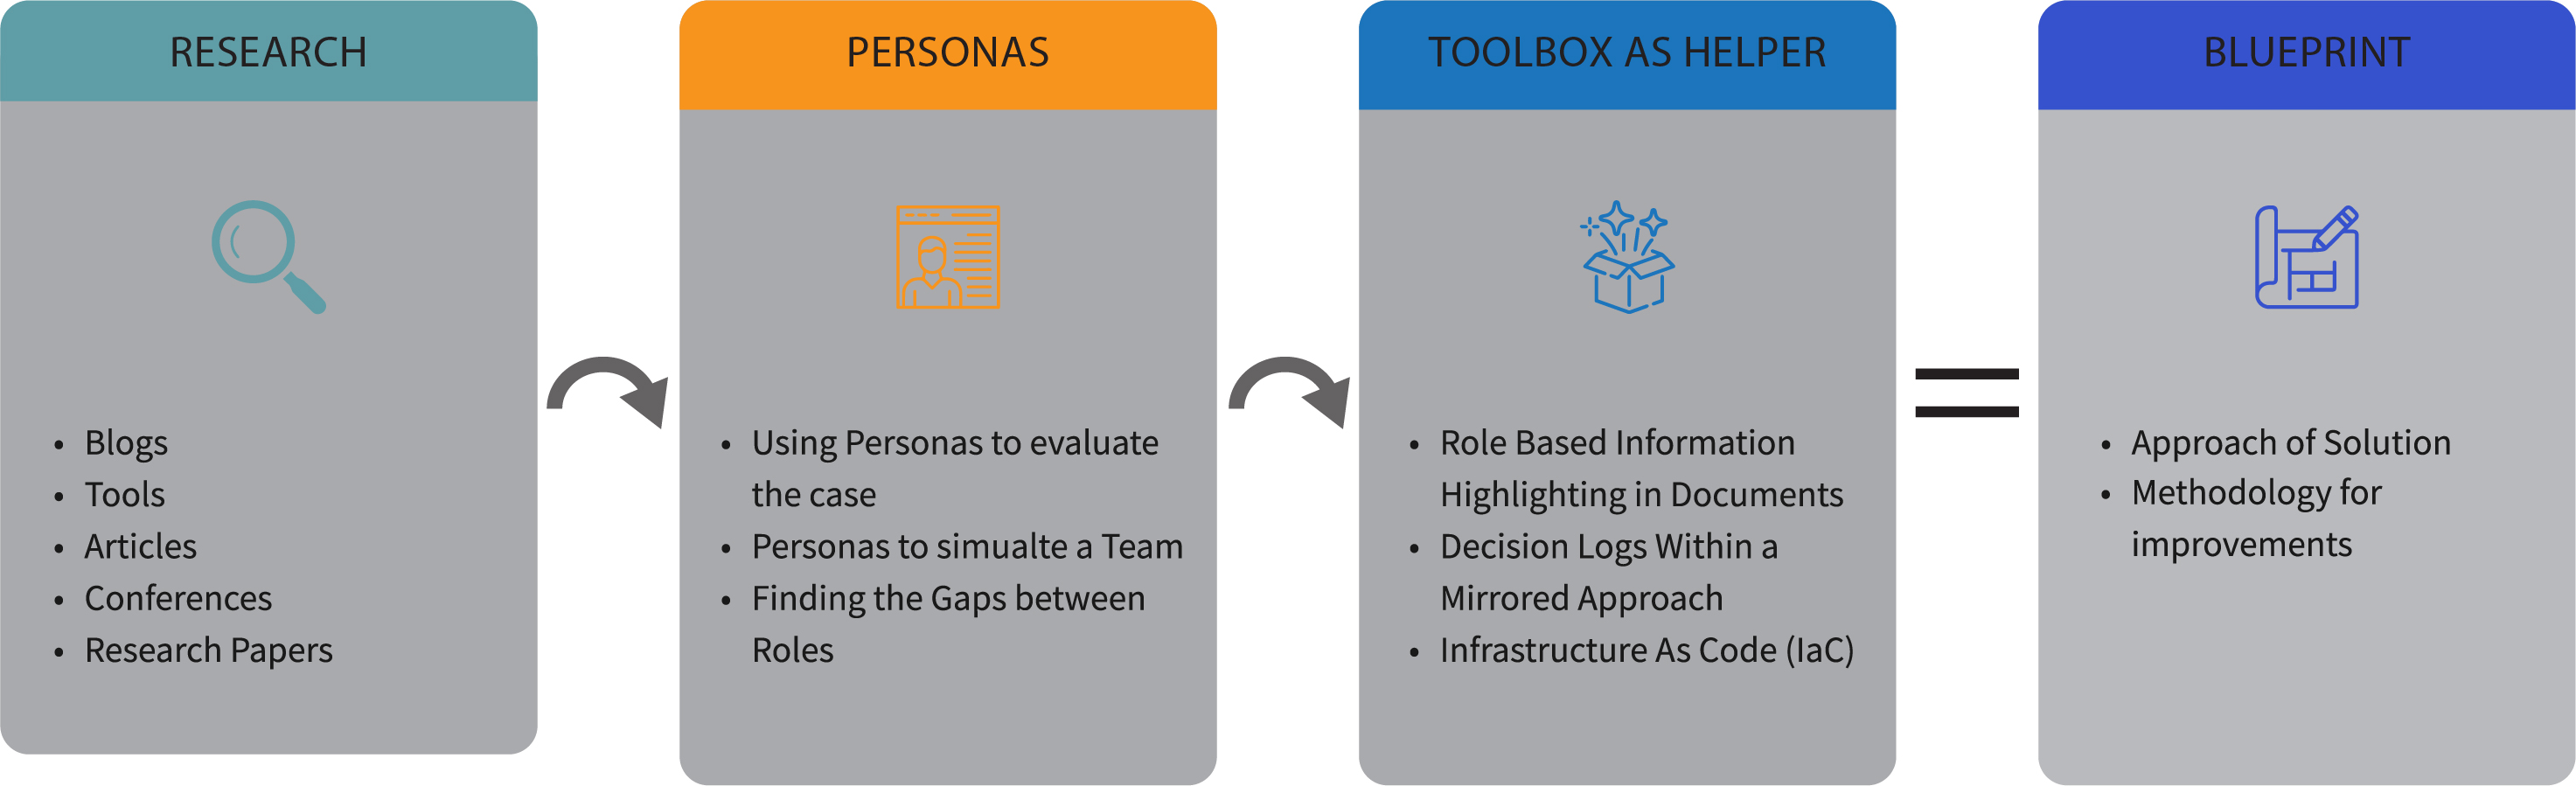
\includegraphics[width=\linewidth]{Images/methodic.jpg}
\caption{Infographic to illustrate Methodology}
\label{fig:methodology:graphic:1}
\end{figure}

\subsection*{Stage 1: Research}
The initial phase of this study comprised a comprehensive analysis of the extant literature in order to establish a solid theoretical foundation. This involved an examination of relevant blogs, tools, articles, conferences and research papers. The objective was to gain an insight into the broader context of knowledge management within \ac{DevOps} environments and to identify any current deficiencies in practice.

\subsection*{Stage 2: Personas}
The utilisation of personas at this stage enabled the simulation of team dynamics and roles in a \ac{DevOps} context. The personas were developed with the objective of evaluating specific use cases and identifying discrepancies between role expectations and reality. The methodology employed facilitated the identification of crucial gaps between various team roles, thereby directing attention to the design of tailored approaches for both documentation and decision-making practices.

\subsection*{Stage 3: Toolbox as Helper}
This phase explored a variety of tools and methodologies that could facilitate the approach of the identified gaps. The focus was on role-based information highlighting within documents, the creation of mirrored decision logs and the integration of \ac{IaC} practices. The aim of this toolbox is to streamline processes and ensure that all team members have access to relevant, up-to-date information. These approaches are then presented to professionals using a survey conducted among software engineering professionals working in a \ac{SCRUM} team.

\subsection*{Stage 4: Blueprint}
The final stage involved the synthesis of all findings, resulting in the formulation of a practical blueprint for the implementation of structured decision logging, along with enhanced knowledge management practices. The blueprint outlines the proposed approach, delineates the roles and responsibilities of various individuals, and suggests methodologies for continuous improvement, with the intention of providing a framework that can be adapted to suit the specific needs of any given context or situation.

\subsection*{Integration with the Visual Representation}

As depicted in Figure \ref{fig:methodology:graphic:1}, the methodology progresses from comprehensive theoretical research to the implementation of specific, actionable strategies. This progression is represented by a structured flow from initial research, through persona development and tool evaluation, and ultimately, to the formulation of a comprehensive blueprint.


%----------------------------------------------------------------------------------------




